\documentclass[10pt,twocolumn,letterpaper]{article}

\usepackage{cvpr2019AuthorKit/latex/cvpr}
\usepackage{times}
\usepackage{epsfig}
\usepackage{graphicx}
\usepackage{amsmath}
\usepackage{amssymb}
\usepackage{xcolor}
\usepackage{algorithm}
\usepackage{algorithmic}
\usepackage{multirow}
\usepackage{arydshln}
\usepackage{subcaption}

\def\x{{\mathsf x}}

% Include other packages here, before hyperref.

% If you comment hyperref and then uncomment it, you should delete
% egpaper.aux before re-running latex.  (Or just hit 'q' on the first latex
% run, let it finish, and you should be clear).
\usepackage[breaklinks=true,bookmarks=false]{hyperref}

\cvprfinalcopy % *** Uncomment this line for the final submission

\def\cvprPaperID{****} % *** Enter the CVPR Paper ID here
\def\httilde{\mbox{\tt\raisebox{-.5ex}{\symbol{126}}}}

% Pages are numbered in submission mode, and unnumbered in camera-ready
%\ifcvprfinal\pagestyle{empty}\fi
\setcounter{page}{1}


%% helper definitions
\def\eg{\emph{e.g.\hspace{0.3em}}}
\def\Eg{\emph{E.g.\hspace{0.3em}}}
\def\ie{\emph{i.e.\hspace{0.3em}}}
\def\etal{\emph{et al.\hspace{0.3em}}}

% TODO
\newcommand{\todo}[1]{}
\renewcommand{\todo}[1]{{\color{red} TODO: {#1}}}

\begin{document}

%%%%%%%%% TITLE
\title{Multi-Task Mutual Learning for Vehicle Re-Identification}

\author{Georgia Rajamanoharan\\
Vision Semantics Ltd\\
{\tt\small georgia@visionsemantics.com}
% For a paper whose authors are all at the same institution,
% omit the following lines up until the closing ``}''.
% Additional authors and addresses can be added with ``\and'',
% just like the second author.
% To save space, use either the email address or home page, not both
\and
Aytac Kanaci \hspace{0.7cm}
%Queen Mary University of London\\
%{\tt\small secondauthor@i2.org}
%\and
Minxian Li  \hspace{0.7cm}
%Queen Mary University of London\\
%{\tt\small secondauthor@i2.org}
%\and
Shaogang Gong\\
Queen Mary University of London\\
{\tt\small \{a.kanaci,m.li,s.gong\}@qmul.ac.uk }
}

\maketitle
%\thispagestyle{empty}

%%%%%%%%% ABSTRACT
\begin{abstract}
Vehicle re-identification (Re-ID) aims to search a specific vehicle
instance across non-overlapping camera views.
%
The main challenge of vehicle Re-ID is that
the visual appearance of vehicles may drastically changes
according to diverse viewpoints and illumination.
%
Most of existing vehicle Re-ID model cannot make full use of
various complementary vehicle information, e.g. vehicle type and orientation.
%
In this paper, we propose a novel {\em Multi-Task Mutual Learning} (MTML) deep model
to learn discriminative features simultaeously from multiple branches.
%
Specially, we design a consensus learning loss function by fusing features from the final convolutional feature maps from all branches.
%
Extensive comparative evaluations demonstrate the effectiveness of our
proposed MTML method in comparison to the state-of-the-art vehicle Re-ID techniques on the a large-scale benchmarks VeRi-776.
We also yield competitive performance on the NVIDIA 2019 AI City Challenge Track 2.
\end{abstract}

%%%%%%%%% BODY TEXT
\section{Introduction}

%%% Background and motivation
%As the ubiquitousness of surveillance cameras capturing vehicle in transport in
%cities and highways increase, the need for analyzing this visual data has
%become an interest in computer vision.

%% Background of vehicle Re-ID
With the development of autonomous driving
and smart city applications, the need to accurately analyze vehicles on urban streets
via multiple computer vision tasks such as detection, classification and
pose estimation, as well as re-identification, is ever-increasing.
%
Specially, vehicle re-identification has attracted increasing attention in the research community
\cite{liu2016vehicleid,liu2016veri,liu2016veri,
wang2017orientation,Wang_2017_ICCV,Zhou2018VAMI},
as it can play an important role in
intelligent transportation systems and public safety.

%% What's vehicle Re-ID?
Vehicle re-identification (Re-ID) aims to search a specific vehicle
instance across non-overlapping camera views.
%
Due to the fact that the license plate is often not visible in a number of view angles (which are generally uncontrolled),
vehicle Re-ID by visual appearance alone is of great practical value in real-world applications such as smart cities.
%
This task is similar to a more popular task: person re-identification
\cite{gong2014re,chen2018person,Li2018Harmonious,xiao2016learning,
li2017person,wei2018person,song2018mask,chang2018multi,
shen2018deep,zhang2017deep,shen2018person,suh2018part},
but with more challenges:
%% Vehicle Re-ID challenges
(1) Unlike person Re-ID, the pose/orientation of vehicles results in occlusion and drastic visual geometry changes, since the vehicle is a kind of rigid body.
% The same vehicle under different viewpoints are visually more diverse than person,
This means that is difficult to infer the same identity from any given pose/orientation of a vehicle.
(2) Even in the same orientation, vehicles of different identities may look very similar
due to the being of the same, or similar, vehicle model. This requires vehicle Re-ID models
to have a more discriminative fine-grained recognition ability.

% Existing work's problem
Most previously proposed vehicle Re-ID methods \cite{liu2016vehicleid,liu2016veri,Shen_2017_ICCV,Zhou2018VAMI} focus on using a single branch
to learn an embedded feature representation for vehicle instance re-identification
from the original information (e.g. the original whole vehicle image).
%
Due to the previously mentioned challenges for vehicle re-identification,
this single branch structure can not take advantage of the diversity of vehicles.
%
Moreover, most existing works
\cite{liu2016vehicleid,liu2016veri}
train their vehicle Re-ID deep learning model
using a single supervisory signal (e.g. vehicle ID).
%
However, we argue that vehicle ID label {\em alone} can not differentiate the differences between vehicles due to the issues we raised above. But additionally we can make use of the fact that the orientation of a vehicle alters its view in a predictable manner.
As a result, we suggest that imposing multiple and different supervisory signals
simultaneously - the vehicle ID \emph{and} vehicle orientation - allows the model to learn this variation in a more well-defined manner, and is thus more effective
for learning the fine-grained discriminative features necessary for vehicle
Re-ID. As orientation labels were provided by Wang \etal \cite{Wang_2017_ICCV} for the VeRi dataset \cite{liu2016veri}, is is possible to make use of these multiple signals for this purpose. Examples of the orientation labels provided by this paper can be seen in Figure \ref{F:veri_veh_orientations}.



\begin{figure*}[t]
  \begin{subfigure}{.6\textwidth}
    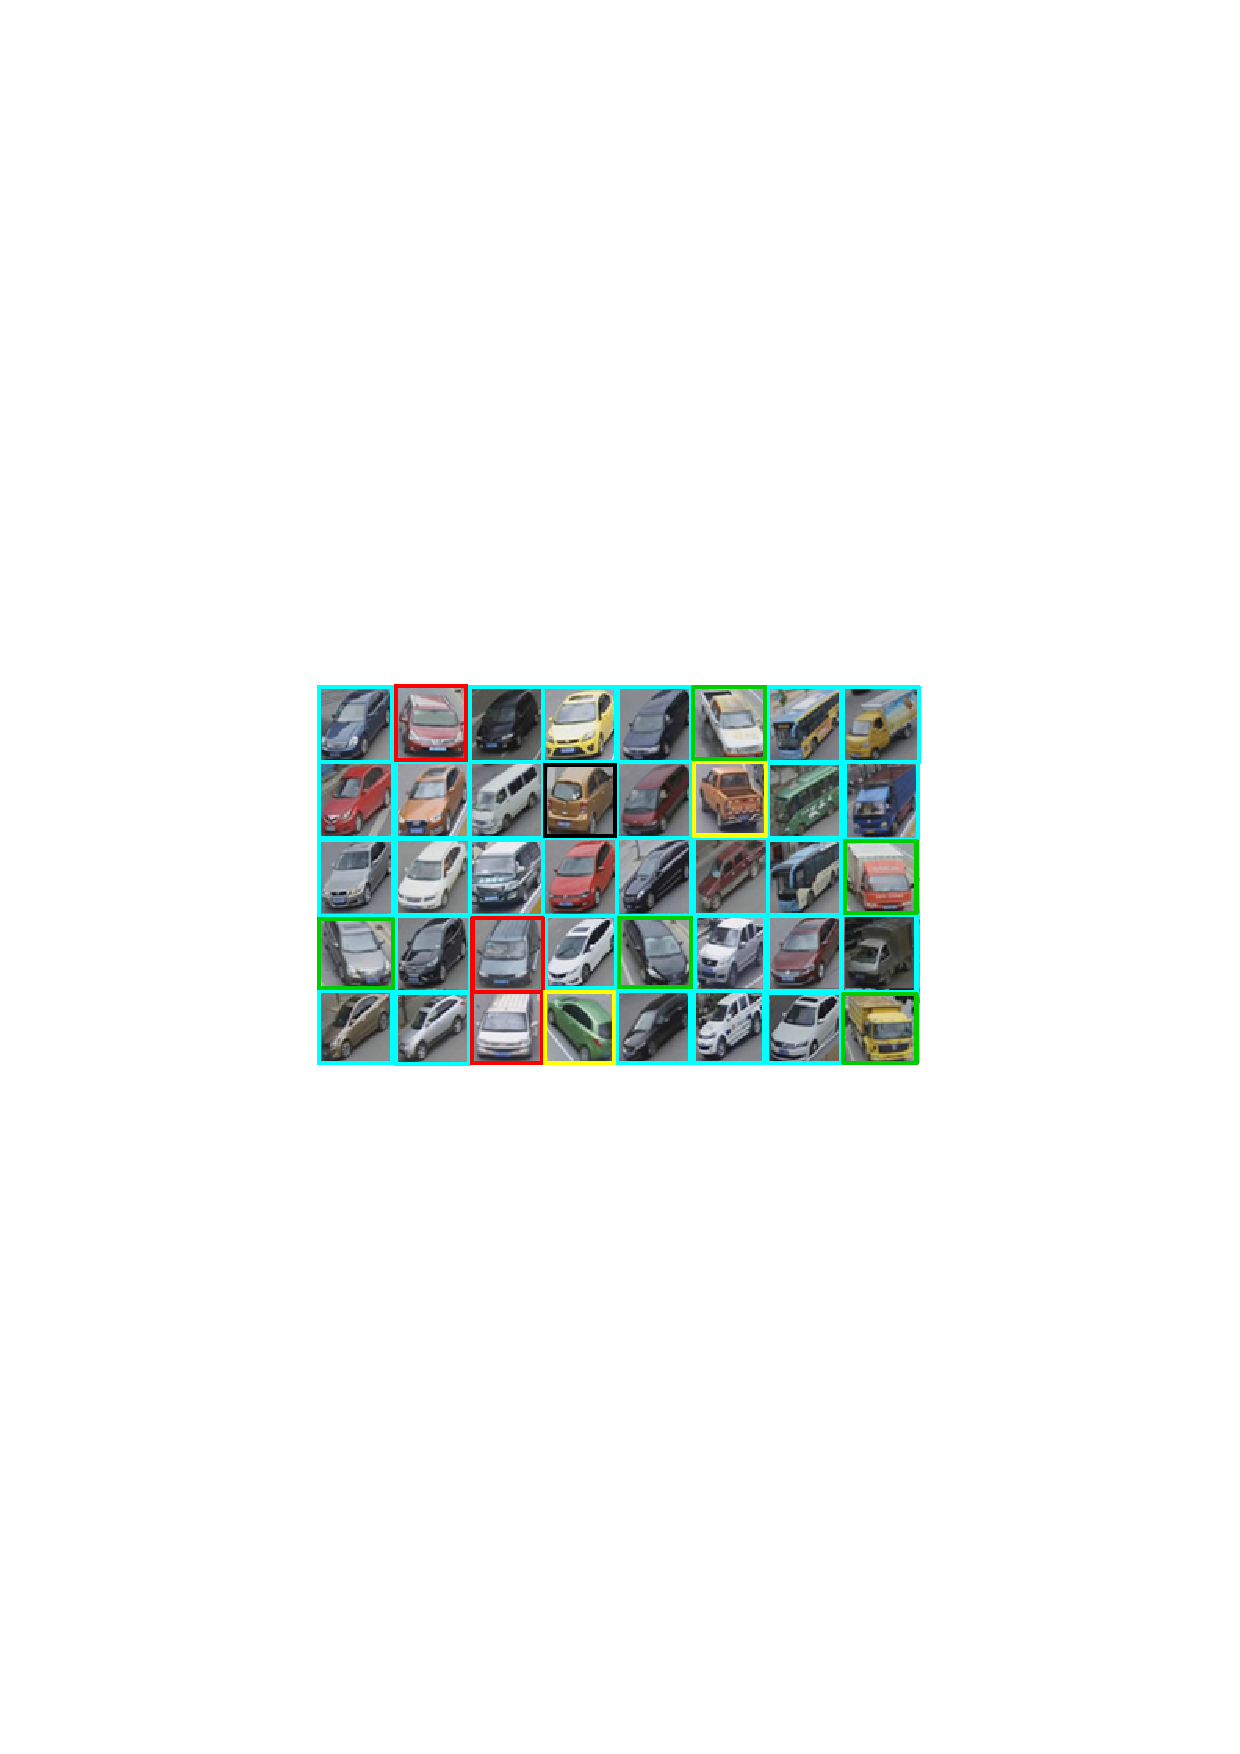
\includegraphics[width=\linewidth,trim=5cm 11cm 5cm 11cm,clip=true]{images/veri_orients.pdf}
  \end{subfigure}
  \begin{subfigure}{.4\textwidth}
    \centering
    \begin{tabular}{c | c | c}
      \hline
      Index & Orientation & Colour \\
      \hline
      0 & front & \textcolor{red}{red} \\
      1 & rear & - \\
      2 & left  & - \\
      3 & left front & \textcolor{cyan}{cyan}  \\
      4 & left rear & \textcolor{yellow}{yellow}  \\
      5 & right  & - \\
      6 & right front & \textcolor{green}{green} \\
      7 & right rear & \textcolor{black}{black} \\
      \hline
    \end{tabular}
  \end{subfigure}
  \caption{Examples from the VeRi776 dataset with the orientation labels provided in \cite{wang2017orientation} (best viewed in colour).}
  \label{F:veri_veh_orientations}
\end{figure*}

%\begin{figure}
%%  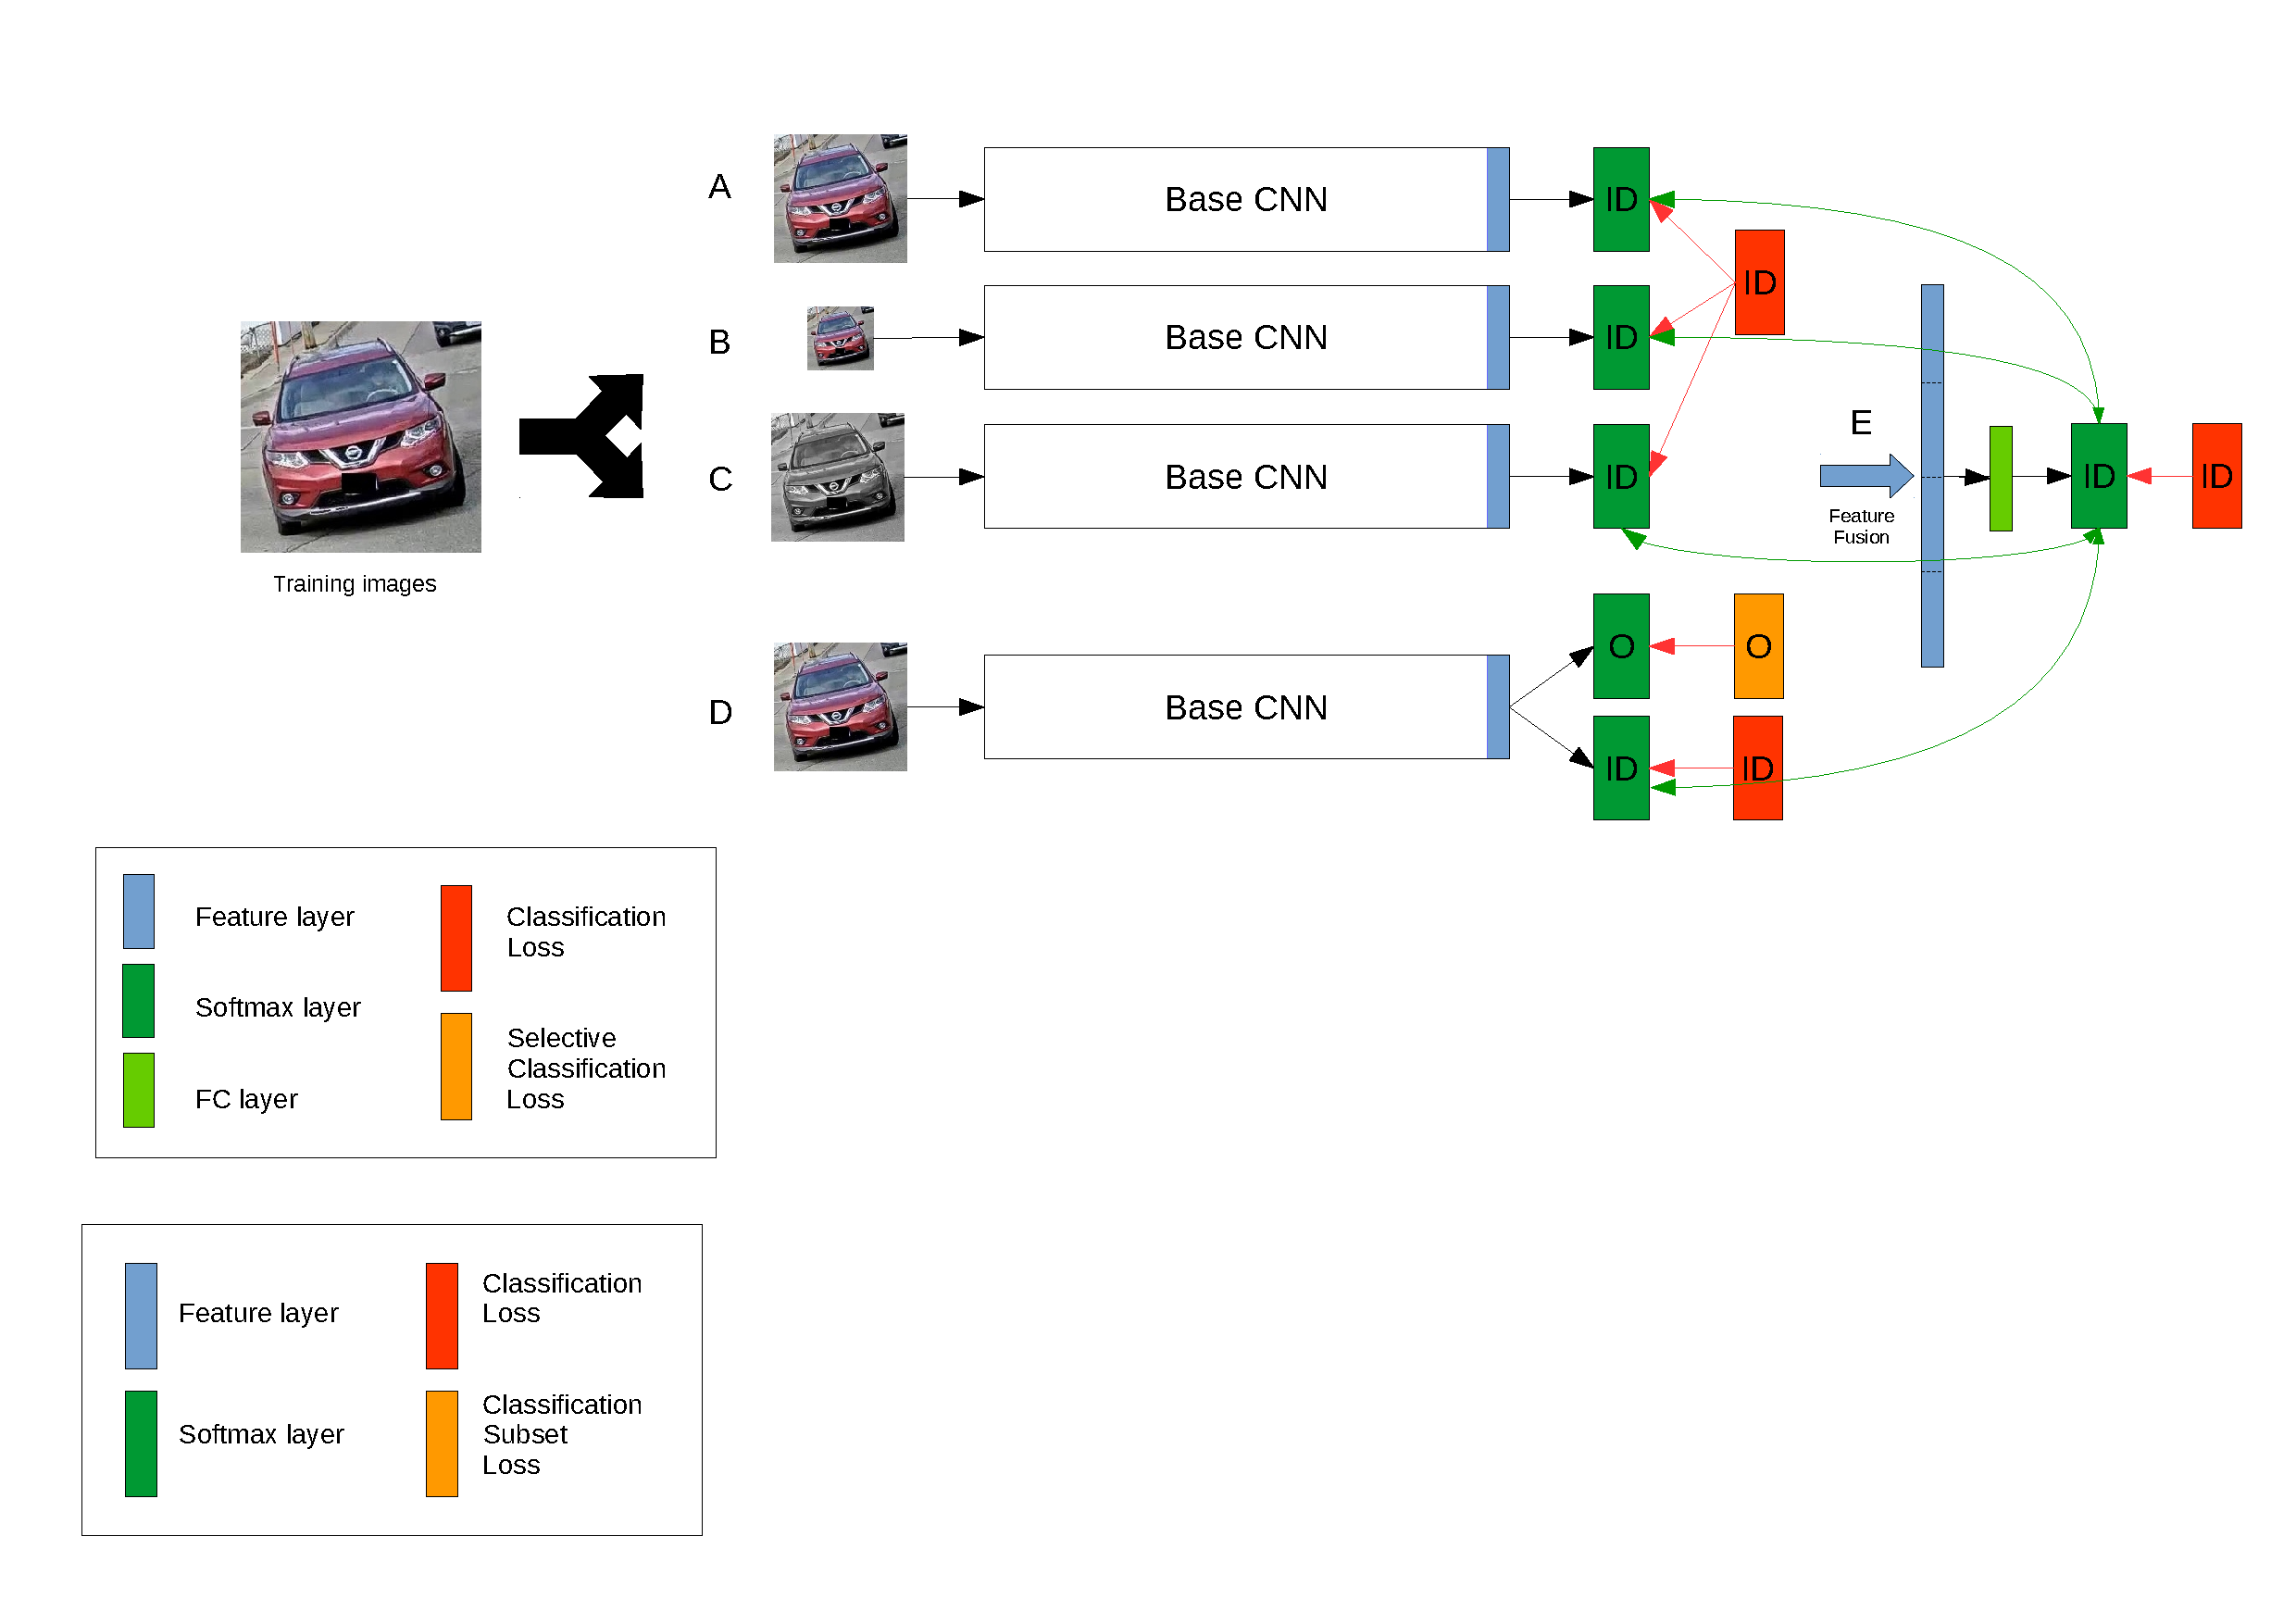
\includegraphics[width=\linewidth,trim=0cm 8cm 0cm 0cm,clip=true]{images/system_overview_orient_only.pdf}
%  \caption{A comparision of the same vehicle ID and different ID.}
%	\label{F:veh_comparison}
%\end{figure}

% Our contributions
In this work, we propose a novel {\em Multi-Task Mutual Learning}
(MTML) based network architecture,
that aims to simultaneously learn a number of recognition tasks from
different supervisory signals, plus a consensus loss function, to
build an improved representation for the purpose of vehicle
re-identification.

We make two contributions in this work as follows:
(1) We formulate a novel {\em Multi-Task Mutual Learning} (MTML) deep
learning model by building each individual branch for a different
recognition task relevant to vehicle Re-ID and by taking into
consideration four different tasks: vehicle ID, multi-scale, grayscale, and orientation.
Our model aims to discover and capture concurrently the complementary discriminative information.
(2) We introduce a mutual learning mechanism for improving multi-task learning robustness.
Our model benefits from multiple supervisory signals in order to
enhance model learning of more discrimative features for vehicle Re-ID.
%(3) we propose a cross-dataset joint learning framework for vehicle Re-ID.
Extensive comparative evaluations demonstrate the effectiveness of the
proposed MTML method in comparison to the state-of-the-art vehicle Re-ID techniques on the a large-scale benchmark
%VehicleID \cite{liu2016vehicleid} and 
VeRi-776 \cite{liu2016veri}.
We also yield competitive performance on the CityFlow
\cite{tang2019cityflow} benchmark at the NVIDIA 2019 AI City Challenge.


%%%%%%%%%%%%%%%%%%%%%%%%%%%%%%%%%
%Generally, vehicle Re-ID task can be regarded as a fine-grained recognition task.
%As a unique ID of a vehicle instance, license plate has been widely used for vehicle Re-ID.
%However, license plate recognition is quite sensitive to image quality,
%camera view and occlusion. Furthermore, license plate may be removed,
%altered even faked in some cases, making it unreliable to identify a vehicle
%simply by its license plate. Therefore, vehicle Re-ID by visual appearance is
%of great practical value in real-world applications such as smart cities.

%Another related problem to vehicle re-identification is fine-grained vehicle model
%classification such as ``Audi A4 2014'' \cite{yang2015compcars}.
%However, the granularity of vehicle re-identification task is much finer
%since the ideal target is to search a specific vehicle rather than a model, in
%which the image instances of the same vehicle (identity) forms a separate class.
%%%% Vehicle Re-ID challenges
%However,
%vehicle Re-ID by visual appearance is a
%challenging task due to the very similar appearance of different vehicle instances
%of the same model type and color, and a significant visual appearance variation
%of the same vehicle instance in different camera views. In other words
%large intra-instance differences of the same vehicle in different cameras,
%and subtle inter-instance differences between different vehicles in the same
%view, considering thousands of vehicles in a large scale smart city setting is
%the main challenge of vehicle Re-ID. Moreover, unlike person Re-ID
%orientation of vehicles results in self occlusion and drastic visual geometry
%changes where in person Re-ID visual geometry or texture of the person's
%appearance (wear) will not change.
% Re-ID problem. A human body is usually upright, thus the texture or color of
% his/her wear will not change severely in different views. Deploying the
% person Re-ID methods for vehicles directly cannot obtain satisfactory
% performance.
% Due to the fact that vehicles are rigid objects, unlike people, the orientation
% of the vehicle can alter very predictably the appearance of in a particular
% viewpoint.

% This area promises the potential for more flexible means for vehicle
% recognition and search than Automatic Number Plate Recognition (ANPR).
% be found as an instance-level object search problem.

%%%% matching probe gallery
%Formally Re-ID  aims to find
%target images of the same identity in a large gallery set given a probe image.
%In order to match appearances of objects, firstly we need to obtain an
%embedding for the objects. A
%match is then performed by using a suitable distance metric expressing the
%closeness of two objects in an embedding space. A good embedding should be
%invariant to illumination, scale and viewpoint changes.

%%%% we use CNNs
%Recently, Convolutional Neural Network (CNN) has achieved state-of-the-art
%performance in various computer vision
%recognition tasks, such as large-scale image classification
%face recognition  and person Re-ID.
%With the supervision of a carefully designed objective loss, typically
%cross-entropy and/or triplet loss
%% contrastive loss or triplet loss
%CNN can learn efficient feature embedding

%%%% Datasets and SOTA
%Influenced by the recent advancements on person Re-ID vehicle Re-ID has started
%to gain increasing attention,
%and a number of vehicle databases and additional labeling are now available to
%facilitate this research
% including
% VeRi-776\cite{Liu2016icme-veri, liu2016veri},
% VehicleID\cite{liu2016vehicleid} and VRIC\cite{kanaci2018vehicle} and methods
% specific to vehicle Re-ID becoming more frequent in various venues
% \cite{wang2017orientation, Shen_2017_ICCV, Zhou2018VAMI}.
%
%%%% Our method:
%\todo{Expand near submission}
%In this paper we propose a new mutual learning based network architecture, that
%aims to simultaneously learn a number of tasks, plus a consensus, to build an
%improved representation for the purpose of vehicle re-identification.
%% Second, we propose to leverage multi-task learning to gen- erate discriminative
%% feature representation by the joint op- timization of group sensitive triplet
%% loss and softmax loss, which can be well applied to accomplish large scale
%% vehicle re-identification towards real applications.
%%%%%%%%%%%%%%%%%%%%%%%%%%%%%%%%%

\section{Related Work}

\noindent {\bf Vehicle Model Classification }
One closely related problem to re-identification is vehicle model
classification
\cite{liao2015exploiting,yang2015compcars,sochor2016boxcars,hu2017deep}.
The two problems are usually studied independently.
For example, Yang et al. \cite{yang2015compcars} propose a part attributes driven
vehicle model recognition.
They also contribute a large comprehensive car dataset named ``CompCars''
with model class labels but without vehicle identity labels.
More recently, Hu et al. \cite{hu2017deep} formulate a deep CNN framework capable of
selecting spatial salient vehicle parts in order to learn more
discriminative model representations without explicit parts annotations.

\noindent {\bf Vehicle Re-Identification. }
%Whist vehicle Re-ID is less studied than person Re-ID
%\cite{gong2014person,li2018harmonious,zhong2017camera},
%there are a handful of existing methods.
%Notably, Feris \etal \cite{feris2012large} proposed an attribute-based Re-ID method.
%The vehicles are firstly classified by different attributes like car model types and colours. The Re-ID matching is then conducted in the attribute space.
%%
%Dominik \etal \cite{zapletal2016vehicle}
%used 3D bounding boxes for rectifying car images and then concatenate colour histogram features of vehicle image pairs.
%A binary linear SVM model is then trained to verify whether a pair of images have the same identity.
%%
%Both methods rely heavily on weak hand-crafted visual features in a
%complex multi-step based approach, suffering from weak discriminative model generalisation.
A number of deep learning techniques have been exploited for the purpose vehicle Re-ID. For instance, Liu
\etal \cite{liu2016veri} explored a deep neural network to estimate the
visual similarities between vehicle images.
%Vehicle appearances, spatio-temporal information and license plates are
%independently and incrementally used to improve the similarity function for
%vehicle matching.  they use a deep neural network to estimate the visual
%similarities between vehicle images for enjoying the strong representation
%learning capacity.
%
Liu \etal \cite{liu2016vehicleid} also designed a Coupled Clusters Loss (CCL)
to boost a multi-branch CNN model for vehicle Re-ID.
%
All these methods utilize the global appearance features of vehicle images and
ignore local discriminative regions.
%
To explore local information motivated by the idea of landmark alignment
\cite{zhang2014facial} in both face recognition \cite{taigman2014deepface} and
human body pose estimation \cite{newell2016stacked}, Wang \etal
\cite{Wang_2017_ICCV} considered 20 vehicle keypoints for learning and aligning
local regions of a vehicle for Re-ID.  Clearly, this approach comes with extra
cost of exhaustively labelling these keypoints in a large number of vehicle
images, and the implicit assumption of having sufficient image
resolution/details for extracting these keypoints.
%

Additionally,
space-time contextual knowledge has also been exploited for vehicle Re-ID
subject to structured scenes \cite{liu2016veri,Shen_2017_ICCV}.
Liu \etal \cite{liu2016veri} proposed
a spatio-temporal affinity approach for quantifying every pair of images.
%This method is inclined to image pairs that are close to each other
%in both spatial and temporal domains therefore only a simplified solution.
%
Shen \etal \cite{Shen_2017_ICCV} further
incorporated spatio-temporal path information of vehicles.
Whilst this method improves the Re-ID performance on the VeRi-776 dataset,
it may not generalize to complex scene structures when the number of
visual spatio-temporal path proposals is very large with only weak contextual
knowledge available to facilitate model decision.

\noindent{\bf Multi-Task Learning. }
Multi-task learning (MTL) is a machine learning strategy
that learns several related tasks simultaneously for
their mutual benefits \cite{argyriou2007multi}. %  \cite{evgeniou2004regularized,ando2005framework,argyriou2007multi}.
A good MTL survey with focus on neural networks
is provided in \cite{caruana1997multitask}.
%
Deep CNNs are well suited for
performing MTL as they are inherently designed to learn joint
feature representations subject to multiple label objectives
concurrently in multi-branch architectures.
%
Joint learning of multiple related tasks
has been proven to be effective in solving computer vision problems
\cite{dong2017multi,zhang2016learning}.
% \cite{dong2017multi,zhang2016learning,ahmed2008training}.
%
Critically, our method is uniquely designed to
explore the potential of MTL
in combining multiple diversities (e.g. scale and color) of the vehicle image
and being supervised by multiple kinds of manual labels (e.g. ID and orientation) with each of them being associated with an individual branch of a single model.


\section{Multi-modal Vehicle Re-identification}

In order to perform Re-ID of previously unseen query vehicles, the aim of our model is to learn a feature embedding that allows for accurate retrivals based on distance (\eg L1) from the query image representation. In order to perform this task, we utilise training data containing a number of different labels: identity class labels as well as vehicle orientation class labels.
%and landmark position labels for a number of specific keypoints
We assume two sets of training examples $\mathcal{I}_1 = \{\mathbf{I_i}\}_{i=1}^N$ and $\mathcal{I}_2 = \{\mathbf{I_i}\}_{i=1}^M$, containing $N$ and $M$ training images respectively. Both training sets contain the associated identity class labels $\mathcal{Y}_1=\{y_i\}_{i=1}^N$ and $\mathcal{Y}_2=\{y_i\}_{i=1}^M$, where $y_i \in \left[1,...,N_{id}\right]$ for $N_{id}$ distinct vehicle idenities spanning the two training sets. However, in addition, $\mathcal{I}_1$ also contains orientation labels, $\mathcal{O_1}=\{o_i\}_{i=1}^N$, where $o_i \in \left[1,...,N_O\right]$ is the orientation (for $N_O$ possible orientations).
%and landmark position labels $\mathcal{L_1}=\{\mathbf{l_i}\}_{i=1}^N$ $\mathbf{l_i}=\{\left(x_{i,1},y_{i,1}\right),...,\left(x_{i,L},y_{i,L}\right)\}$ defines the position of $N_L$ keypoint landmarks for the vehicle within image $\mathbf{I}_i$, which we normalise according to the image size so that $x,y \in [0,1]$

In order to perform accurate Re-ID, we use this data to build a model constructed from multiple branches, each of which is tasked with learning a specific aspect of the data concurrently. The branches of the model are as follows: A) Identity classification B) Identity classification from a scaled image C) Identity from grayscale image D) Identity plus the vehicles' orienations.
These individual branches then form a consensus prediction on the identity of the training examples, and this consensus is then employed for regulation of the individual branches.

\subsection{Model Structure and Feature Learning}

\begin{figure*}
  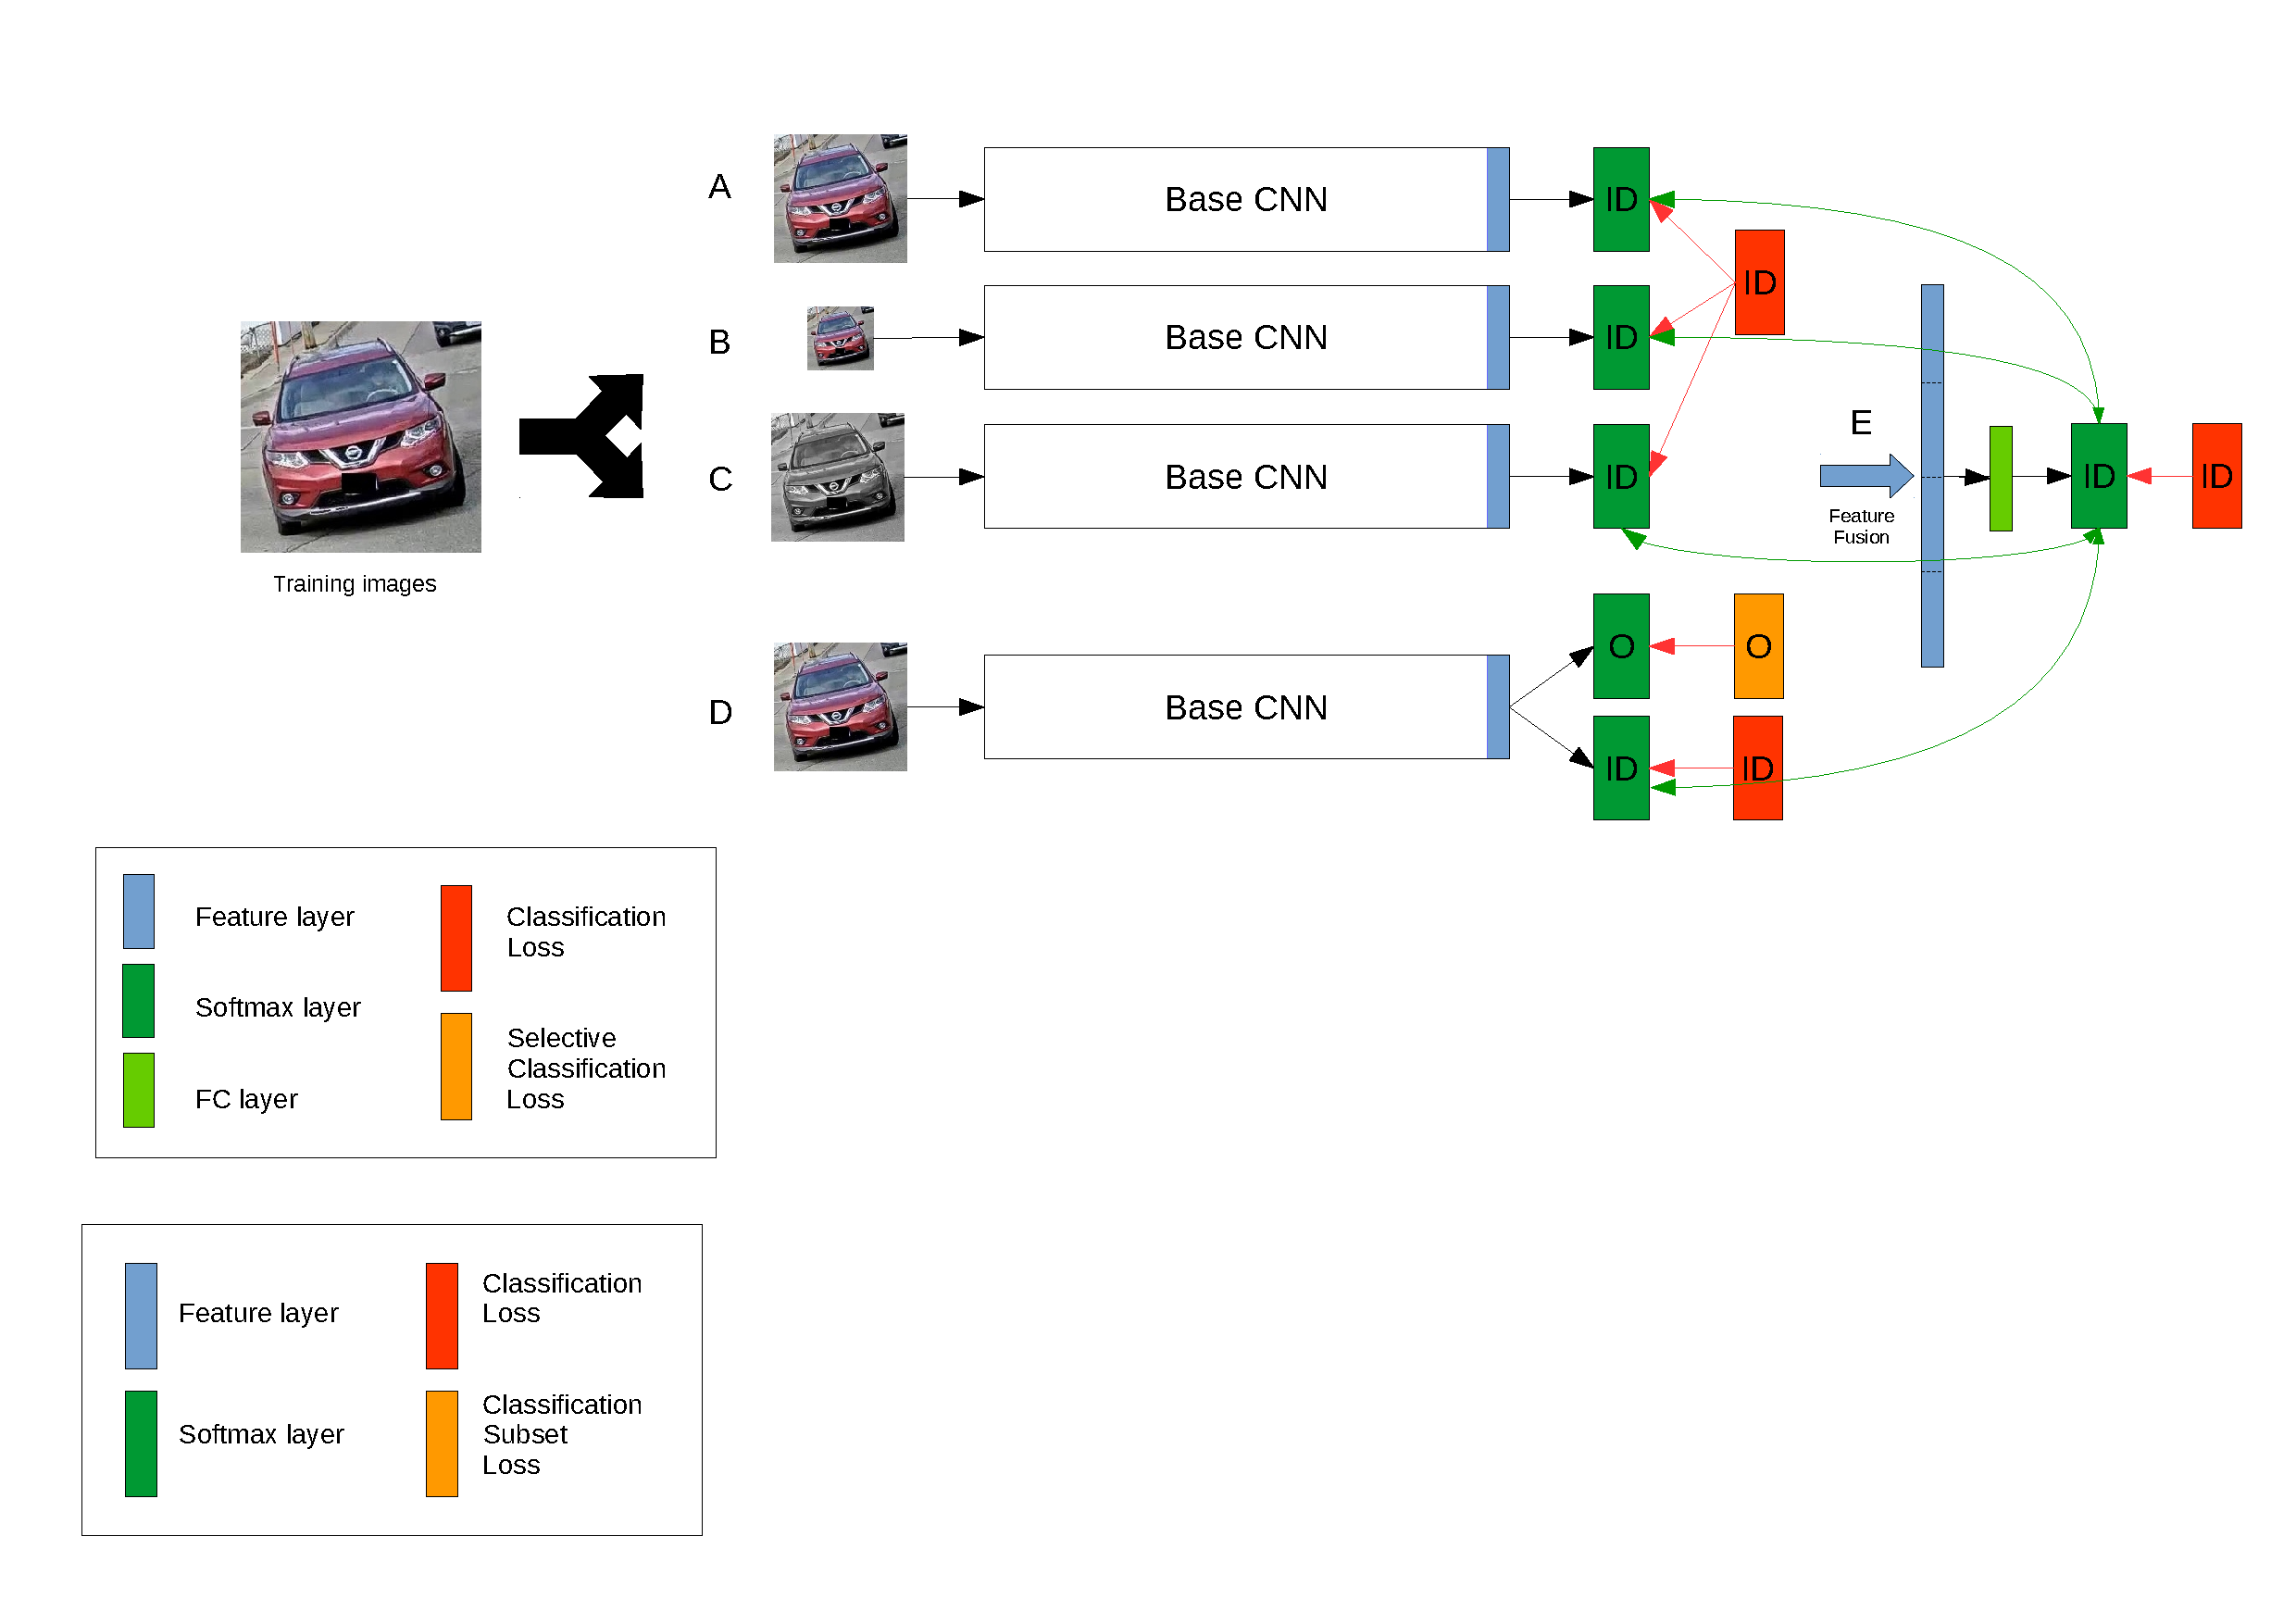
\includegraphics[width=\linewidth,trim=0cm 8cm 0cm 0cm,clip=true]{images/system_overview_orient_only.pdf}
  \caption{An overview of our proposed model (best viewed in colour). (A) Vehicle identity branch (B) Multi-scale analysis branch (C) Grayscale analysis branch (D) Vehicle orientation branch
    %(E) Vehicle landmark localisation branch.
(E) Consensus learning through feature fusion. Feedforward signals shown in black. Hard target (groundtruth) loss propagation shown in \textcolor{red}{red}. Soft target consensus feedback loss propagation shown in \textcolor{green}{green}.}
  \label{F:overview}
\end{figure*}

An overview of our proposed model can be seen in Figure
\ref{F:overview}. The model is composed of four sub-branches, each of
which is simultaneously learning a representation to solve its own
task. In addition, there is a single fusion branch, which allows
feature selection to be performed from the entire collection of
individual representations. It is the output from this branch that is
taken during deployment. Each sub-branch will now be described in more
detail.

\paragraph{(A) Vehicle Identity}

The root branch of our model is tasked with learning the best representation for vehicle identity discrimination, for both training sets $\mathcal{I}_1$ and $\mathcal{I}_2$.
Here, we exploit the cross entropy classification loss function in order to train one branch to predict vehicle identity. Thus the branch calculates the softmax posterior probability of the class label $y_i$ for a given training image $\mathbf{I_i}$:
\begin{equation}
  p_i^{ID} = p(\hat{y_i} = y_i|\mathbf{I_i}) = \frac{\exp(\hat{y_i})}{\sum_{k=1}^{N_{id}}\exp(\hat{y_k})}
  \label{E:softmax_id}
\end{equation}
where $\hat{y_k} = \mathbf{w_k^Tx_i}$, $\mathbf{x_i}$ is the feature vector for image $\mathbf{I_i}$ given by final layer of the branch, and $\mathbf{w_k}$ is the prediction function parameter for identity class $\emph{k}$. The loss across a minibatch of $N_B$ images can then be computed as:
\begin{equation}
  L_{ID} = -\frac{1}{N_B} \sum_{i=1}^{N_B} \log{p_i^{ID}}
  \label{E:cross_entropy_loss}
\end{equation}

\paragraph{(B) Identity from Scaled Image}

Here we exploit the multi-scale analysis that has previously been shown to be of benefit for the task of re-identification, both for persons \cite{chen2017person} and vehicles \cite{kanaci2018vehicle}. This is done by including a branch that is trained via cross entropy loss (Eq. \ref{E:cross_entropy_loss}) to predict the class identity from a rescaled version of the input image, in a similar way to branch A.

\paragraph{(C) Identity from Grayscale Image}

In order to encourage the model to focus on details of the vehicles,
that allow for separation of highly similar identity classes, we
ensure that one branch will be unable to use colour information for
distinguishing between these classes. This is done by giving as input
only the grayscale image, and again training the branch to predict
identity via the cross entropy loss.

\paragraph{(D) Vehicle Orientation}

This branch is tasked with learning a representation to simultaneously
predict the identity class and the orientation class when this is known.
%In the case where the training images do not have associated orientation labels, this branch is trained in exactly the same way as the Vehicle Identity branch outlined above.
Both sets of labels are simultaneously employed in a joint loss function in order to optimise the branch for prediction of both identity and orientation. As orientation labels are not available for all training data, we employ a selective classifcation subset loss function, that allows the loss to be calculated across only the subset of the batch for which orientation labels are known.

Again, the cross entropy loss is exploited for this task. Hence, the branch calculates both Eq. (\ref{E:softmax_id}), as well as the softmax posterior probability of the orientation label $o_i$ for the images for which the orientation class is known:
\begin{equation}
  p_i^{O} = p(\hat{o_i} = o_i|\mathbf{I_i}) = \frac{\exp(\hat{o_i})}{\sum_{j=1}^{N_{O}}\exp(\hat{o_j})}
\end{equation}
where this time $\hat{o_j} = \mathbf{w_j^Tx_j}$, and $\mathbf{w_j}$ is the prediction function parameter for orientation class $\emph{j}$.

The loss for this branch is then calculated across the minibatch of images as:
\begin{equation}
  L_{O} = -\frac{1}{N_B} \sum_{i=1}^{N_B}\log{p_i^{ID}} + \frac{1}{N_S} \sum_{i=1}^{N_B}q_i^O
\end{equation}
where $N_S$ is the size of the subset of the minibatch for which orientation labels are known, and
\[
q_i^O =
\begin{cases}
    \log{p_i^{O}} & \text{if } o_i \in \mathcal{O} \\
    0 & \text{otherwise}
\end{cases}
\]
%% \paragraph{(E) Vehicle Landmark Localisation}

%% Vehicle landmarks are distinguishing features that must be employed in order to perform correct  re-identification of vehicles that look very similar. Hence it is crucial that our model picks up on these in its feature representation. In order to attempt to ensure this, we task one branch with simultaneously predicting the position of these landmarks (if present) as well as the identity class. As above, if no landmark labels are available in the minibatch, this branch is trained in exactly the same way as branch A.

%% If landmark groundtruth labels are available, these are employed to train the branch to predict the location of the landmarks which are present, while at the same time predict identity. As a different set of landmarks are visible, depending on the orientation of the vehicle, we need to take the absence of landmarks altogether into account when training this branch. Thus, we design a loss function that only penalises the predictions for landmarks that are present in the groundtruth labels for the minibatch examples. As this is the regression problem, we also set the final layer of the branch to output with linear activation, and take the Mean Squared Error (MSE) as the basis for our custom loss function. If the landmarks were all present in every training image, we could use the standard MSE loss:
%% \begin{equation}
%%   M = \frac{1}{N_B} \sum_{j=1}^{N_L} \sum_{i=1}^{N_B} (\hat{x_{i,j}} - x_{i,j})^2 + (\hat{y_{i,j}} - y_{i,j})^2
%% \end{equation}
%% where $\hat{x_{i,j}}$ and $\hat{y_{i,j}}$ are the predicted normalised coordinates. However, we need to alter this to remove landmarks that are not present at all in the image. Hence we design a selective MSE function that only takes into account those landmarks which the groundtruth labels indicate are present in the image. Thus:
%% \begin{equation}
%%   M = \sum_{j=1}^{N_L} \frac{1}{N_{B_j}} \sum_{i \in B_j} (\hat{x_{i,j}} - x_{i,j})^2 + (\hat{y_{i,j}} - y_{i,j})^2
%% \end{equation}
%% where $B_j$ is the subset of the minibatch examples for which landmark $j$ is present in image $\mathbf{I_i}$. Due to the nature of the landmarks, we can assume that there will be a similar number of examples in the batch that contain each landmark, hence we can approximate this as:
%% \begin{equation}
%%   M = \frac{1}{\bar{N_{B_j}}} \sum_{j=1}^{N_L}  \sum_{i \in B_j} (\hat{x_{i,j}} - x_{i,j})^2 + (\hat{y_{i,j}} - y_{i,j})^2
%% \end{equation}
%% where $\bar{N_{B_j}}$ is the mean number of examples containing each landmark, in order to simplify the calculation. Then the full loss function for the landmark branch becomes:
%% \begin{equation}
%%   l_{LM} = M - \frac{1}{N_B} \sum_{i=1}^{N_B} \log{p_i}
%% \end{equation}

\paragraph{(E) Consensus Learning and Feedback}

In order to harness the benefit of all branches for the purpose of vehicle re-identification, we employ consensus learning as proposed in \cite{chen2017person} and previously harnessed for vehicle Re-ID in \cite{kanaci2018vehicle}. This is done via feature fusion of the final convolutional feature maps from all branches for consensus learning. As our branches are based on the ResNet50 architecture \cite{he2016deep}, these feature maps are formed via an average pooling operation which result in feature vectors of length $2048$. Hence our fused features are of length $8192$. We then add one additional fully connected layer, of size $1024$, and the output of this passed to a final identity softmax classification layer, again employed with cross entropy loss. Hence:
\begin{equation}
  p_i^C = p(\hat{y_i^C} = y_i|\mathbf{I_i}) = \frac{\exp(\hat{y_i^C})}{\sum_{k=1}^{N_{id}}\exp(\hat{y_k^C})}
\end{equation}

Additionally, we also utilise a consensus propagation mechanism, similar to the previously proposed method \cite{chen2017person,kanaci2018vehicle}. Here the consensus output is taken as `soft targets' (as opposed to the groundtruth label `hard targets') for the training data, and used to feedback information about the predictions made by the entire ensemble of branches. This is done concurrently with the training of the individual branches. Thie method is inspired by the idea of Knowledge Distillation (KD) \cite{hinton2015distilling}, but is different in that here we employ the combined predictions from all the `student' branches as a \emph{virtual} teacher model, rather than utilising a pre-trainined powerful teacher model to provide the soft targets.

Specifically, the feedback mechanism employs the consensus probability predictions $P^C_i = \left[p_{i,1}^C,...,p_{i,j}^C,...,p_{i,N_{ID}}^C\right]$ given image $\mathbf{I_i}$, feeding these into the cross entropy loss between the two distributions to provide a consensus regularisation loss for the branch:
\begin{equation}
  \mathcal{H}_i = \mathcal{H}(P^C_i, P_i) = -\frac{1}{N_{ID}}\sum_{j=1}^{N_{ID}} p_j^c \log{p_j}
\end{equation}
The total consensus loss for a particular branch is then:
\begin{equation}
  L_{C} = \frac{1}{N_B} \sum_{i=1}^{N_B} \mathcal{H}_i
\end{equation}
This is added to each individual branch's loss functions. In addition, this mechanism provides regularisation of the whole network by propagating all of the consensus losses back through the feature fusion layer, which also boosts the learning of the ensemble.

\subsection{Model Training}

In order to train our model, we combine both training sets, $\mathcal{I}_1$ and $\mathcal{I}_2$, and employ batches that contain both images with and without orientation labelling. The full training algorithm can be seen in Algorithm \ref{A:model_training}.

\begin{algorithm}[t]
  \begin{algorithmic}
    \REQUIRE{Training sets $\mathcal{I}_1$ $\mathcal{I}_2$, labels $\mathcal{Y}_1$ $\mathcal{Y}_2$\
      $\mathcal{O}_1$, model $\mathcal{M}$}
    \STATE{$\bullet$ Initialise network branches with pre-trained ImageNet weights}
    \STATE{$\bullet$ Initialise output layers of $\mathcal{M}$ randomly}

    \FOR{epoch $e \in (1, E)$}

        \STATE{$\bullet$ Feed-forward through model to obtain all branch identity classification \
          predictions on images in $\mathcal{I}_1$ and $\mathcal{I}_2$}
        \STATE{$\bullet$ Feed-forward to obtain orientation classification predictions on $\mathcal{I}_1$}
        \STATE{$\bullet$ Fuse features and perform consensus identity classification predictions on both training sets}
        \STATE{$\bullet$ Calculate hard and soft losses identity losses for each branch and backpropagate to update weights}
        \STATE{$\bullet$ Calculate orientation losses using labels for $\mathcal{I}_1$ and backpropagate to update weights on the orientation branch}
        \STATE{$\bullet$ Calculate hard and soft identity losses for the consensus branch and backpropagate}
     \ENDFOR

  \end{algorithmic}
  \caption{The MTML training algorithm.}
  \label{A:model_training}
\end{algorithm}

\subsection{Vehicle Re-ID deployment}

During deployment, we employ the feature fusion layer from our trained model as the full feature representation in order to perform vehicle re-identification matching. As we do not necessarily have camera information about the query or gallery images, or timestamp information, which would allow the use of camera distance or time-based analysis, we use only a generic distance metric - the $L1$ metric - in order to match gallery images to the query. Hence, for each of the query image $\mathbf{I}^q$, and the gallery images $\{\mathbf{I}_i^g\}$,  we compute our $6400$ dimension fused feature representations, $\mathbf{x}^q$ and $\{\mathbf{x}_i^g\}$ respectively. We then calculate the $L1$ distance between the query representation and each of the gallery images, and rank the latter by increasing distance in order to calculate the Rank-1 and mAP performance scores.

%\subsection{Re-ranking}
%\emph{TODO}

\begin{table*}
  \centering
  \begin{tabular}{c || c | c | c || c | c || c | c}
    \hline
    \multirow{2}{*}{Dataset} & \multicolumn{3}{c||}{Training} & \multicolumn{2}{c||}{Probe} & \multicolumn{2}{c}{Gallery} \\
    \cline{2-8}
    & \#IDs& \#Imgs & \#Orients & \#IDs & \#Imgs & \#IDs & \#Imgs \\
    \hline
    VeRi-776 \cite{liu2016veri}
    & 576 & 37778 & 8 & 200 & 1678 & 200 & 11579 \\
%     VehicleID \cite{liu2016vehicleid}
%     & 13164 & 100182 & - & 2400 & 17638 & 2400 & 2400 \\
%    BoxCars \cite{} & 21250 & 63750 & -  & - & - & - & - \\
%    CompCars \cite{} & 1118 & 31148 & - & - & - & - & - \\
    CityFlow \cite{tang2019cityflow}
    & 333 & 36935 & - & 333 & 1052 & 333 & 18290 \\
    \hline
  \end{tabular}
  \caption{Details of the datasets employed for train and test.}
  \label{T:dataset_details}
\end{table*}





\section{Experiments}

\begin{table}[h]
  \centering
  \begin{tabular}{l || c | c | c }
    \hline
    Method & mAP & Rank-1 & Rank-5 \\
    \hline
    MSVF \cite{kanaci2018vehicle} & 49.3 & 88.6 & - \\
    OIFE \cite{wang2017orientation} & 51.4 & 68.3 & 89.7 \\
    S-CNN+P-LSTM \cite{Shen_2017_ICCV} & 58.3 & 83.5 & 90.0 \\
    MTCRO \cite{xu2018framework} & 61.6 & 87.2 & 94.2 \\
    MTCRO (ReRank) \cite{xu2018framework} & 62.6 & 88.0 & 94.6 \\
    \hline
    MTML-S & 59.4 & 89.5 & 94.9 \\
    MTML-O & 60.8 & 90.2 & 95.4 \\
    MTML-G & 62.8 & 91.1 & 95.8 \\
    \hline
    MTML-SG & 63.7 & 90.6 & 95.8 \\
    MTML-OG & 63.5 & 92.0 & \bf{96.4}\\
    MTML-OSG & \bf{64.6} & \bf{92.3} & 95.7 \\
    MTML-OSG (ReRank) & \bf{\emph{68.3}} & 92.0 & 94.2 \\
    \hline
  \end{tabular}
  \caption{Trained/tested on VeRi776 only}
  \label{T:benchmark_results_veri}
\end{table}

We conduct a number of experiments to explore the performance of our method. First we exploit a number of widely available vehicle ID benchmark datasets in order to assess the benefit of each of the branches of our model independently, and altogether. Then we compare the performance of our model to other current work by looking at our performance in the NVIDIA AI City Challenge 2019 Task 2 (Vehicle Re-identification). As our method includes a branch that predicts vehicle orientation in addition to identity, our model requires data that contains the orientation labels for training. As a result, we include the VeRI776 \cite{liu2016veri} dataset in the training set for all our experiments.


\subsection{Datasets}
We employ two Vehicle Re-ID datasets in our experiments, in order to train and test our method extensively. Firstly we conduct experiments on a benchmark dataset, VeRi776 \cite{liu2016veri}, which has been widely tested by the majority of recent works. And secondly we employ the new CityFlow dataset \cite{tang2019cityflow}, a challenging dataset that has been shown to be more difficult than previous publicly available benchmarks.
%
The VeRi-776 dataset \cite{liu2016veri} has 37,778 images of 576 IDs in the training set and 200
IDs in the test set. The standard probe and gallery sets consist of 1,678 and 11,579
images, respectively. There are also orientation labels, for 8 possible orientations, available for the VeRi-776 dataset, which were provided by \cite{Wang_2017_ICCV}.
%
%% The VehicleID \cite{liu2016vehicleid} dataset provides a training set with 113,346 from 13,164 IDs and a test set
%% with 19,777 images from 2,400 identities. It adopts the single-shot re-id setting,
%% with only one true matching for each probe. Following the standard setting, we
%% repeated 10 times of randomly selected probe and gallery sets in our experiments.
%
The CityFlow dataset \cite{tang2019cityflow} has 36,935 images of 333 IDs in the training set and 333 different IDs in the test set. The standard probe and gallery sets consist of 1,052 and 18,290 images respectively.
The data split statistics of both datasets are summarised in Table \ref{T:dataset_details}.

\subsection{Implementation Details}
We employ the ResNet50 \cite{he2016deep} network
architecture as the base of our model. We train the model with
minibatches of size 8, using the Adam optimisation technique with a
learning rate of 0.0001, exponential decay rates set as follows:
$\beta_1=0.9$ and $\beta_2=0.999$. The two image sizes used were
standard $224\x224$ and small (for the scaled branch) $160\x160$.

We measure the performance of our vehicle re-identification methods according to the standard Cumulative Matching Characteristic (CMC) and mean Average Precision (mAP). The CMC is computed on each individual rank $k$ as the cumulative percentage of correct matches appearing
at ranks $\leq k$. The mAP is calculated as the mean over all query images of the Average Precision, which itself is calculated as the precision cut-off at each correct recalled image position averaged over all possible correct gallery images.

\subsection{Evaluation on Veri776 Dataset}
Firstly, we train and test on the VeRi776 dataset in order to compare with
existing state-of-the-art methods with identical settings. In order to experiment the benefit of adding each of the separate branches of our model, we take branch A (vehicle identity) as our central branch, and of course all models have an E consensus branch, and then perform experiments where we include each of the other branches in turn. So MTML-S refers to a model built from branches A, B and E only, MTML-G has branches A, C and E only, and so on. We then test versions of the model with three branches (e.g. MTML-SG includes branches A, B, C and E).  
MTML-OSG (branches A, B, C, D and E) is then our full model, and MTML-OSG (ReRank \cite{zhong2017re}) the results of the full model after additional re-ranking. Table \ref{T:benchmark_results_veri} shows the results of this
experiment, with all experiments run for 150 epochs of training. As can be seen,
even before re-ranking, our full model achieves state-of-the-art mAP
and Rank-1 scores on this dataset, of 64.6\% and 92.3\%
respectively. And after re-ranking the mAP score is increased to an
impressive 68.3\%.

The mAP results from the experiments also show how the individual branches contribute to the performance, with orientation (60.8\%) improving over the result of scaled analysis alone (59.4\%), and grayscale doing even better (62.8\%). This demonstrates how allowing the model to learn about the orientation of the vehicle at the same time as identity can strengthen the performance. And that removal of the colour during learning - though obviously a useful indicator of identity at test time - allows for the model to focus on the more discriminatory features of the identity that ultimately boosts the re-id performance.

The combinations of three branches all show improvement over only two, with MTML-SG and MTML-OG achieving mAPs of 63.7\% and 63.5\% respectively. However they are still outperformed by combining all four branches in the MTML-OSG model. These results show that combining all the different signals for MTL does indeed allow for the overall model to perform better in the final task of vehicle re-identification.

%\textcolor{red}{TODO more detailed discussion of results}

%% \subsection{Evaluation on the VehicleID Dataset}
%% Second, we then train on both the VeRi776 and VehicleID datasets, and
%% test on VehicleID with all three of its test sets: small, medium and
%% large. We conducted this experiment to explore the benefit of training
%% model using additional orientation labels, as VeRi776 is the only
%% dataset available with orientation labels.

%% \textcolor{red}
%% {
%% Table \ref{T:benchmark_results_vehicleid} shows that ...
%% (Please add some comparison methods in Table 3)
%% }
%% ({\bf SG: missing results})

%\begin{table}
%  \centering
%  \setlength{\tabcolsep}{0.01cm}
%  \begin{tabular}{l || c | c || c | c || c | c }
%    \hline
%    \multirow{2}{*}{Method} & \multicolumn{2}{c}{Small} & \multicolumn{2}{c}{Medium} &\multicolumn{2}{c}{Large} \\
%    \cline{2-7}
%    & mAP & Rank-1 & mAP & Rank-1 & mAP & Rank-1 \\
%    \hline
%    MTML-S & \\
%    MTML-O & \\
%    MTML-G & \\
%    % \hdashline
%    MTML-SG & \\
%    MTML-OG & \\
%    MTML-OSG & \\
%    % \hdashline
%    MTML-OSG+ReRank & \\
%    \hline
%  \end{tabular}
%  \caption{Trained on VeRi776+VehicleID, tested on VehicleID}
%  \label{T:benchmark_results_vehicleid}
%\end{table}

\subsection{Evaluation on CityFlow Dataset}

\begin{table}[h]
  \centering
  \begin{tabular}{l || c | c | c }
    \hline
    Method & mAP & Rank-1 & Rank-5 \\
    \hline
    Resnet50 \cite{tang2019cityflow} & 25.5 & 41.3 & - \\
    \hline
    MTML-S  & 17.0 & 40.4 & 53.3 \\
    MTML-G  & 19.6 & 44.5 & 58.4 \\
    \hdashline
    MTML-SG & 20.6 & 44.1 & 55.8 \\
    \hdashline
    MTML-SG (ReRank) &  & & \\
    \hline
  \end{tabular}
  \caption{Trained/tested on CityFlow}
  \label{T:cityflow_results}
\end{table}


\begin{table}[h]
  \centering
  \setlength{\tabcolsep}{0.05cm}
  \begin{tabular}{l|c|c|c|c|c|c}
  \hline
  \multicolumn{1}{r|}{Test:} & \multicolumn{3}{c|}{VeRi-776} & \multicolumn{3}{c}{CityFlow} \\
  \hline
  Method       & mAP   & Rank-1  & Rank-5  & mAP   & Rank-1 & Rank-5  \\
  \hline
  MTML-O       &       &         &         &       &        &         \\
  MTML-S       &       &         &         &       &        &         \\
  MTML-G       & 61.6  & 89.7    & 95.1    & 22.3  & 47.4   & 57.3   \\
  MTML-SG      & 62.6  & 90.8    & 95.8    & 23.0  & 46.6   & 60.5   \\
  MTML-OG      &       &         &         &       &        &         \\
  MTML-OSG     &       &         &         &       &        &      \\
  \hline
  \end{tabular}
  \caption{Trained/tested on CityFlow+VeRi-776}
  \label{T:cf_veri_res}
\end{table}

We participated in Task 2 of the NVIDIA AI City Challenge 2019. The aim of this task was attempt city-scale multi-camera vehicle re-identification. Multiple cameras were placed at multiple intersections and no camera information was provided about the images.

Two groups of experiments are conducted on CityFlow benchmark: 
(1) Training on CityFlow, and (2) Training on CityFlow and Veri-776.
%
For the first group experiment, we trained MTML-S (branch A, B and E), 
MTML-G (branch A, C and E) and MTML-SG model only on CityFlow training data.
Table \ref{T:cityflow_results} shows that: 
(1) -G branch combination is much better than -S branch combination. 
The potential reason is that grayscale analysis is more useful than mult-scale in vehicle Re-ID.
(2) Joint learning with -S and -G is better than any individual one of them on mAP evaluation.

%The reason of combine Veri-776 dataset into training set is that
Since the orientation label is only available in Veri-776, 
for training the full MTML model including orientation supervisory signal,
we did the second group experiment.
%
%Table \ref{T:cf_veri_res} shows that: 




%\begin{table}
%  \centering
%  \begin{tabular}{l || c | c}
%
%  \end{tabular}
%  \caption{}
%  \label{T:aicity_results}
%\end{table}

\section{Conclusions}
Vehicle Re-ID is difficult because the visual appearance of
a vehicle instance may drastically change due to diverse
viewpoints and illumination, whilst different vehicle instances of the same
model type may have a very similar appearance.
%
In this paper, we propose a novel {\em Multi-Task Mutual Learning} (MTML) deep model
to learn discriminative feature simultaeously from multiple branches.
%
Moreover, we design a consensus learning loss function by fusing feature of the final convolutional feature maps from all branches.
%
Extensive comparative evaluations demonstrate the effectiveness of the
proposed MTML method in comparison to the state-of-the-art vehicle Re-ID techniques on the a existing large-scale benchmarks VeRi-776.
%VehicleID and
We also yield a competitive performance on the NVIDIA 2019 AI City Challenge Track 2.

{\small
\bibliographystyle{cvpr2019AuthorKit/latex/ieee_fullname}
\bibliography{bibliography}
}

\end{document}
